%%
%% Automatically generated file from DocOnce source
%% (https://github.com/hplgit/doconce/)
%%
%%


%-------------------- begin preamble ----------------------

\documentclass[%
twoside,                 % oneside: electronic viewing, twoside: printing
final,                   % or draft (marks overfull hboxes, figures with paths)
10pt]{article}

\listfiles               % print all files needed to compile this document

\usepackage{relsize,makeidx,color,setspace,amsmath,amsfonts}
\usepackage[table]{xcolor}
\usepackage{bm,microtype}

\usepackage{graphicx}

\usepackage[T1]{fontenc}
%\usepackage[latin1]{inputenc}
\usepackage{ucs}
\usepackage[utf8x]{inputenc}

\usepackage{lmodern}         % Latin Modern fonts derived from Computer Modern

% Hyperlinks in PDF:
\definecolor{linkcolor}{rgb}{0,0,0.4}
\usepackage{hyperref}
\hypersetup{
    breaklinks=true,
    colorlinks=true,
    linkcolor=linkcolor,
    urlcolor=linkcolor,
    citecolor=black,
    filecolor=black,
    %filecolor=blue,
    pdfmenubar=true,
    pdftoolbar=true,
    bookmarksdepth=3   % Uncomment (and tweak) for PDF bookmarks with more levels than the TOC
    }
%\hyperbaseurl{}   % hyperlinks are relative to this root

\setcounter{tocdepth}{2}  % number chapter, section, subsection

% Tricks for having figures close to where they are defined:
% 1. define less restrictive rules for where to put figures
\setcounter{topnumber}{2}
\setcounter{bottomnumber}{2}
\setcounter{totalnumber}{4}
\renewcommand{\topfraction}{0.85}
\renewcommand{\bottomfraction}{0.85}
\renewcommand{\textfraction}{0.15}
\renewcommand{\floatpagefraction}{0.7}
% 2. ensure all figures are flushed before next section
\usepackage[section]{placeins}
% 3. enable begin{figure}[H] (often leads to ugly pagebreaks)
%\usepackage{float}\restylefloat{figure}

\usepackage[framemethod=TikZ]{mdframed}

% --- begin definitions of admonition environments ---

% --- end of definitions of admonition environments ---

% prevent orhpans and widows
\clubpenalty = 10000
\widowpenalty = 10000

% --- end of standard preamble for documents ---


% insert custom LaTeX commands...

\raggedbottom
\makeindex

%-------------------- end preamble ----------------------

\begin{document}

% endif for #ifdef PREAMBLE


% ------------------- main content ----------------------



% ----------------- title -------------------------

\thispagestyle{empty}

\begin{center}
{\LARGE\bf
\begin{spacing}{1.25}
Education for the future
\end{spacing}
}
\end{center}

% ----------------- author(s) -------------------------

\begin{center}
{\bf Morten Hjorth-Jensen${}^{1, 2}$} \\ [0mm]
\end{center}

    
\begin{center}
{\bf Anders Malthe-Sørenssen${}^{1}$} \\ [0mm]
\end{center}

    \begin{center}
% List of all institutions:
\centerline{{\small ${}^1$Department of Physics, University of Oslo}}
\centerline{{\small ${}^2$Department of Physics and Astronomy, Michigan State University, USA}}
\end{center}
    
% ----------------- end author(s) -------------------------

\begin{center} % date
September 2 2015, 
\end{center}

\vspace{1cm}


% !split
\subsection*{How we perceive the role of education, present and future}

% --- begin paragraph admon ---
\paragraph{}
The main topics of this talk are:

\begin{itemize}
\item \textbf{Research-based education}, from undergraduate studies to a PhD: \href{{http://www.mn.uio.no/fysikk/english/research/groups/computational/index.html}}{The Computational Physics group at the University of Oslo} as example

\item Future challenges and directions
\end{itemize}

\noindent
% --- end paragraph admon ---



% --- begin paragraph admon ---
\paragraph{Takeaway message.}
A successful research program cannot be disconnected from education and vice versa
% --- end paragraph admon ---



% !split
\subsection*{The role of computations, from education to society}

% --- begin paragraph admon ---
\paragraph{}
\textbf{Computations of almost all systems in science are central to our
basic understanding of nature and technological advances}.
% --- end paragraph admon ---



% --- begin paragraph admon ---
\paragraph{Examples.}
\begin{itemize}
\item \textbf{Nanotech and Materials}: quantum physical systems in nanotechnology; characteristics of new materials; semi-conductor devices and quantum computers 

\item \textbf{The smallest particles in nature}: subatomic physics at its smallest length scale

\item \textbf{And the largest}: simulating galaxies and the evolution of the universe

\item \textbf{Life science}: cancer treatment and how the brain works

\item \textbf{Geosciences}: predicting climate changes and this week's weather, simulating natural disasters

\item \textbf{Finance}: assessing risk in the insurance and financial industry

\item and many many more
\end{itemize}

\noindent
% --- end paragraph admon ---



% !split
\subsection*{Modeling and computations as a way to enhance algorithminc thinking}

% --- begin paragraph admon ---
\paragraph{}
\textbf{Algorithm} : A finite set of unambiguous instructions that, given some set of initial conditions, can be performed in a prescribed sequence to achieve a certain goal.
% --- end paragraph admon ---




% --- begin paragraph admon ---
\paragraph{}
\textbf{Algorithmic  thinking as a way to} :
\begin{itemize}
\item Enhance instruction based teaching

\item Introduce research-based teaching  from day one

\item Trigger further insights in math and other disciplines 

\item Validation and verification of scientific results, with the possibility to emphasize ethical aspects as well. Version control is central

\item Good working practices from day one
\end{itemize}

\noindent
% --- end paragraph admon ---





% !split
\subsection*{What do we mean with computing?}

% --- begin paragraph admon ---
\paragraph{}

\textbf{Computing means solving scientific problems using computers. It covers numerical as well as symbolic computing. Computing is also about developing an understanding of the scientific process by enhancing algorithmic thinking when solving problems.}

And this  competence is about:

\begin{itemize}
\item derivation, verification, and implementation of algorithms

\item understanding what can go wrong with algorithms

\item overview of important, known algorithms

\item understanding how algorithms are used to solve complicated problems

\item reproducible science and ethics

\item algorithmic thinking for gaining deeper insights about scientific problems
\end{itemize}

\noindent
All these elements (and many more) aid students in maturing and gaining a better understanding of the scientific process \emph{per se}.
% --- end paragraph admon ---







% !split
\subsection*{Computing and research-based education}

% --- begin paragraph admon ---
\paragraph{}
A computational approach allows us to introduce research concepts and engage students in research from \emph{day one}.
% --- end paragraph admon ---



% --- begin paragraph admon ---
\paragraph{How do we define research-based education?}
It is fully integrated with a direct participation in actual research and builds upon established
knowledge and insights about scientific methods.
% --- end paragraph admon ---





% !split
\subsection*{Research-based education}

% --- begin paragraph admon ---
\paragraph{What should the education contain?}
The standard situation we meet at an almost daily basis:

\begin{itemize}
\item Theory+experiment+simulation is almost the norm in research and industry

\item To be able to model complex systems with no simple answers. Solve real problems.

\item Emphasis on insight and understanding of fundamental principles and laws in the Sciences.

\item Be able to visualize, present, discuss, interpret and come with a critical analysis of the results, and develop a sound ethical attitude to own and other's work.

\item Enhance reasoning about the scientific method
\end{itemize}

\noindent
Our education should reflect this. An example where this takes place is the \href{{http://www.mn.uio.no/fysikk/english/research/groups/computational/index.html}}{Computational Physics group at UiO}.  How can we implement in a systematic was a research-based education?
% --- end paragraph admon ---




% !split
\subsection*{\href{{http://www.mn.uio.no/fysikk/english/research/groups/computational/index.html}}{Computational Physics group at UiO}; implementing our visions}

% --- begin paragraph admon ---
\paragraph{}
A particular strength of physics students is their ability to pose and
solve problems that combine physical insights with mathematical
and  computational skills. This provides a unique combination
of applied and theoretical knowledge and skills. These features are invaluable 
for the development of multi-disciplinary educational and research programs for future challenges.
% --- end paragraph admon ---




% !split
\subsection*{Develop a social, scientific and learning environment}

% --- begin paragraph admon ---
\paragraph{}
\begin{itemize}
\item \textbf{The main aim is that students should realize their own potentials and creative power}
\begin{itemize}

 \item Students come with different dreams, ambitions, aspirations and topics they wish to study, our approach is to tailor the education to all these, an possibly more, aspects

 \item Our motto is to foster students which are better than their supervisors. This is how we define progress

 \item This creates an atmosphere for learning and sharing knowledge

 \item The emphasis is on learning and getting new insights. Students and teachers help each other

 \item No competing environment but a drive and enthusiam in sharing and developing new knowledge

 \item This creates an enviroment where students with different backgrounds and needs can thrive socially and scientifically

\end{itemize}

\noindent
\item \textbf{Takeaway message: Developing a collaborative educational environment is central for multi-disciplinary research projects to succeed}
\end{itemize}

\noindent
% --- end paragraph admon ---





% !split
\subsection*{Develop a social, scientific and learning environment}

% --- begin paragraph admon ---
\paragraph{}
\begin{itemize}
\item The computational physics group includes bachelor, master of science and doctoral students

\item Project oriented work where students develop and mature their own ideas, with an individually tailored approach to each students

\item Office space with desktops to every student and large common room for recreational activities (meals, common lunches, gaming, watching movies etc etc)

\item Many students collaborate on similar  thesis topics and \href{{http://www.dn.no/talent/2014/06/12/Utdannelse/sommervikar-ble-toppforsker}}{publish in top scientific journals}
\end{itemize}

\noindent
% --- end paragraph admon ---





% !split
\subsection*{Developing a good learning environment}

% --- begin paragraph admon ---
\paragraph{}
\begin{itemize}
\item Our students have made significant contributions to  the \href{{http://www.mn.uio.no/english/about/collaboration/cse/}}{Computing in Science Education}  (UiO education prize in 2011) by developing exercises and participating in educational projects at the MN faculty

\item Our students have also developed educational \href{{http://www.mn.uio.no/fysikk/om/aktuelt/aktuelle-saker/2015/realfagsapper.html}}{tools and applications for understanding complicated physical problems} 

\item The students keep shaping and developing the scientific, social and pedagogical activities of the group

\item A group of PhD students is now developing \href{{https://github.com/CINPLA/ibvcse}}{new textbooks for Computational Life Science}

\item During the last ten years more than 60 students have finalized their master theses in computational physics and  almost 60\% have continued with PhD studies

\item Many students don't want to leave the group after finishing their studies
\end{itemize}

\noindent
% --- end paragraph admon ---






% !split
\subsection*{Investing in equipment for students}

% --- begin paragraph admon ---
\paragraph{Using research funds for visualization tools.}


% inline figure
\centerline{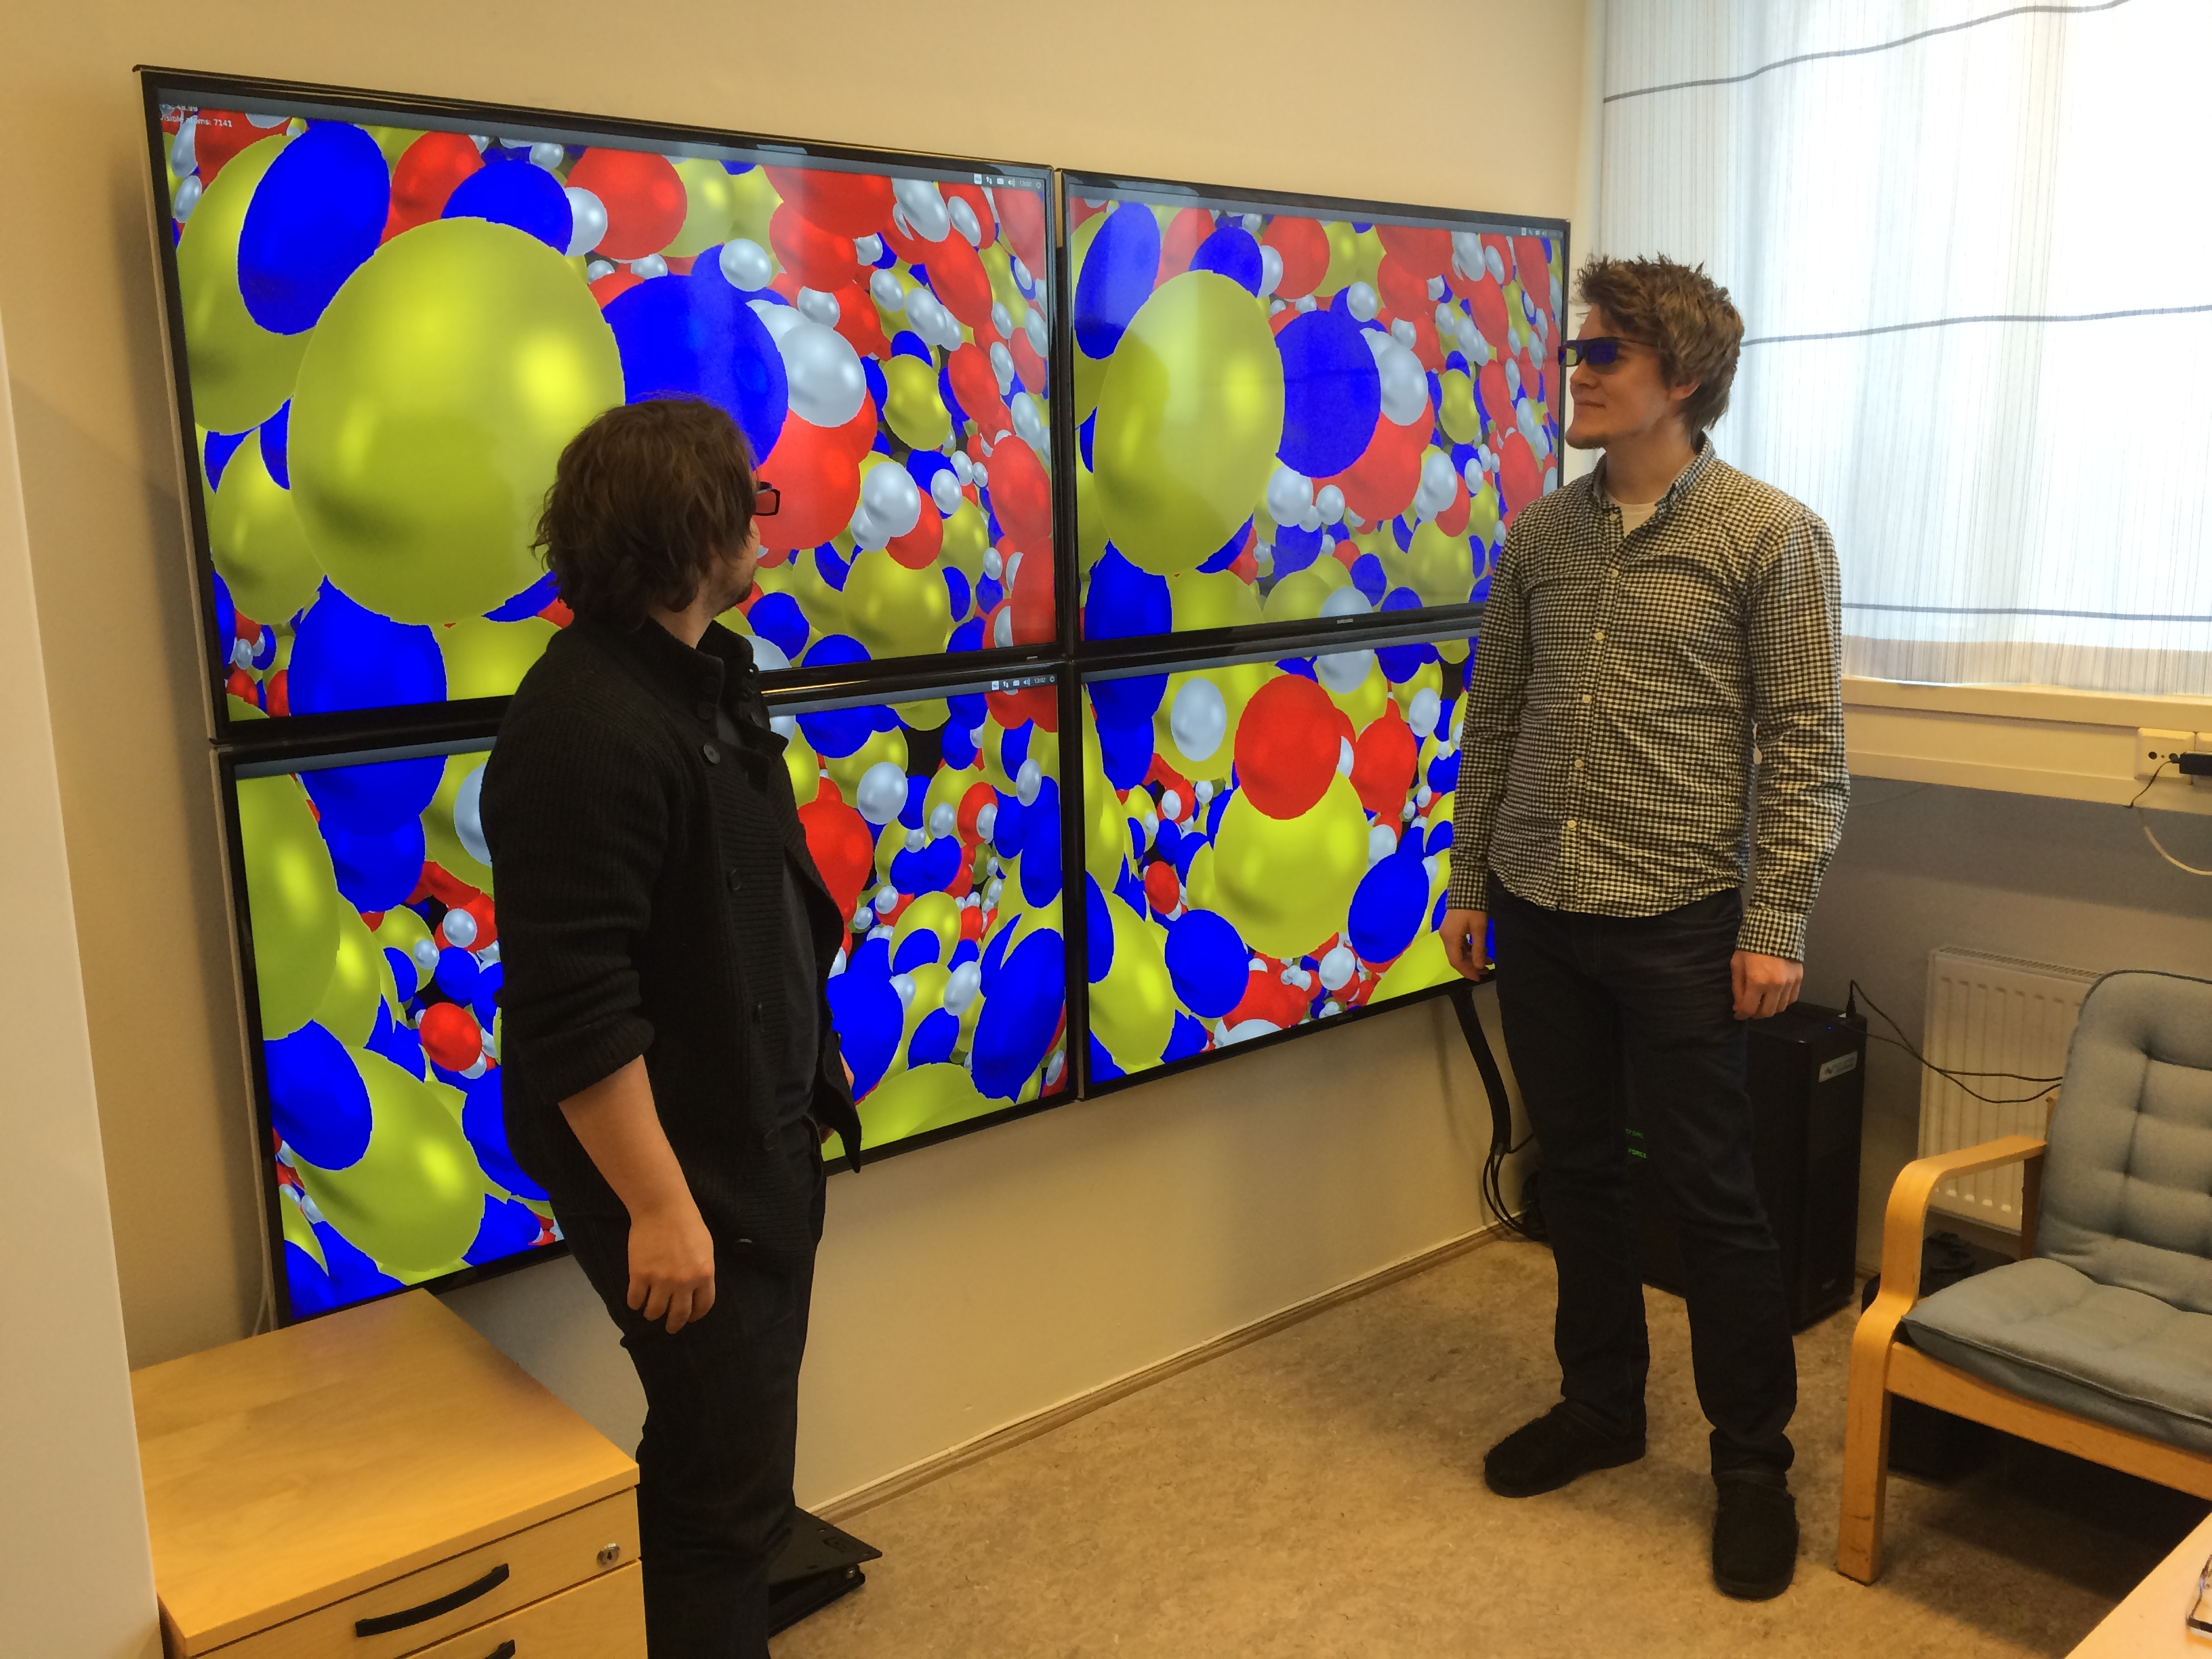
\includegraphics[width=0.7\linewidth]{fig-future/visualize.jpg}}
% --- end paragraph admon ---




% !split
\subsection*{Building a supercomputing cluster}

% --- begin paragraph admon ---
\paragraph{We got (for free) the old supercomputer at UiO (TITAN).}


% inline figure
\centerline{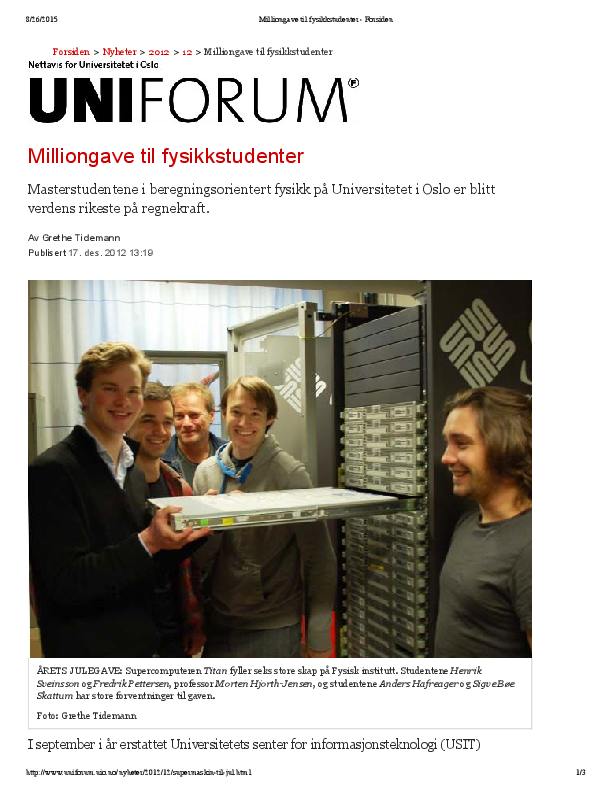
\includegraphics[width=0.7\linewidth]{fig-future/uniforum-0.png}}
% --- end paragraph admon ---




% !split
\subsection*{Undergraduate student publishes in PNAS}

% --- begin paragraph admon ---
\paragraph{Using research funds for visualization tools.}


% inline figure
\centerline{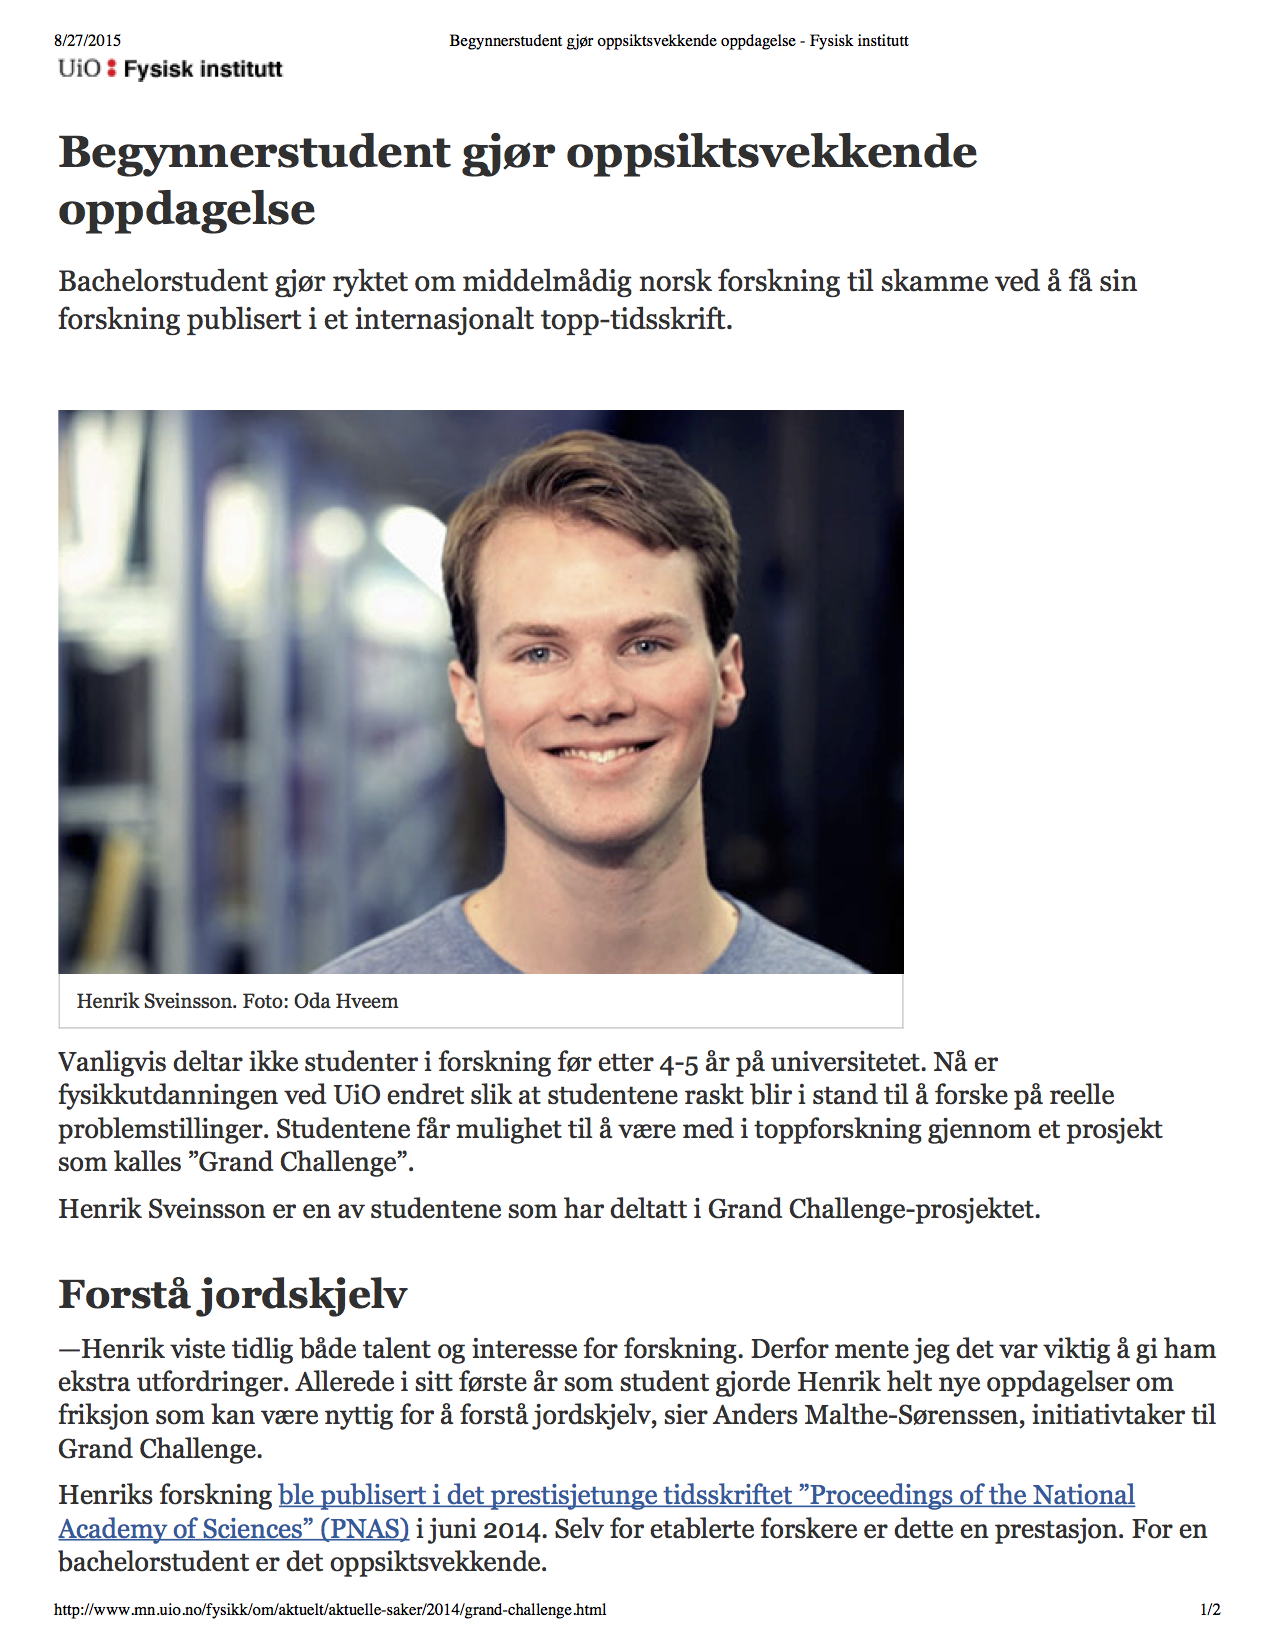
\includegraphics[width=0.7\linewidth]{fig-future/pnas.png}}
% --- end paragraph admon ---






% !split
\subsection*{The future: Multiscale modeling is the big open research question}


% --- begin paragraph admon ---
\paragraph{}
Present and future problems, unlike traditional
science and engineering, involve complex systems with many distinct
physical processes. 
\begin{itemize}
\item The wide open research topic of this century, both in industry and at universities, is how to effectively couple processes across different length and energy scales. 

\item Progress will rely on a multi-disciplinary approach and therefore the  need for multi-disciplinary educational and research programs.
\end{itemize}

\noindent
% --- end paragraph admon ---




% --- begin paragraph admon ---
\paragraph{}
We need to foster candidates with the right
multi-disciplinary background and computational thinking for
understanding present and future simulation technologies and their challenges.
% --- end paragraph admon ---




% !split
\subsection*{Examples of large scale simulations}

% --- begin paragraph admon ---
\paragraph{Fluid dynamical simulations central in air industry.}


% inline figure
\centerline{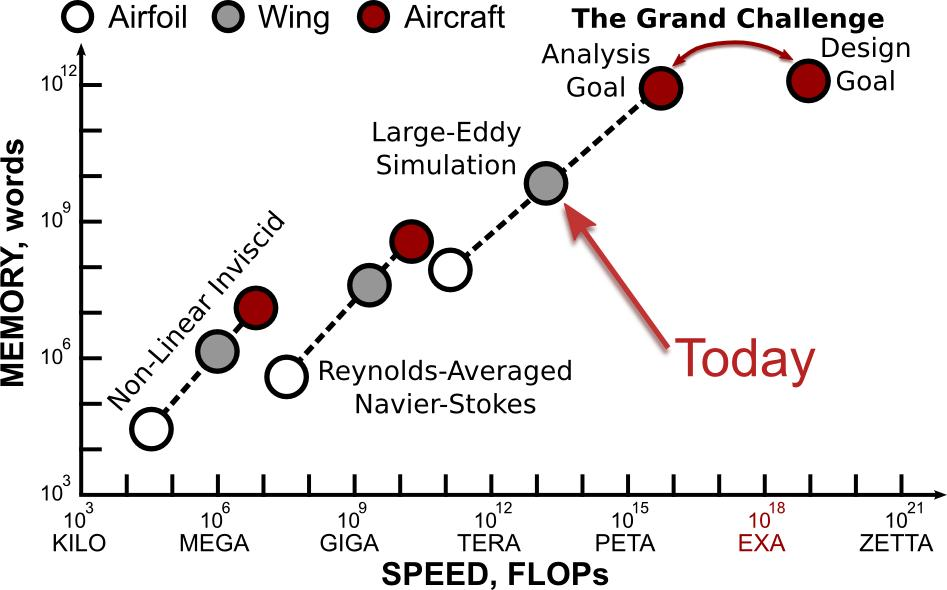
\includegraphics[width=0.6\linewidth]{fig-future/fig10.jpg}}
% --- end paragraph admon ---




% !split
\subsection*{Testing plane wings via massive numerical simulations}

% --- begin paragraph admon ---
\paragraph{}
Fluid dynamical simulations central in air industry, wings tested.


% inline figure
\centerline{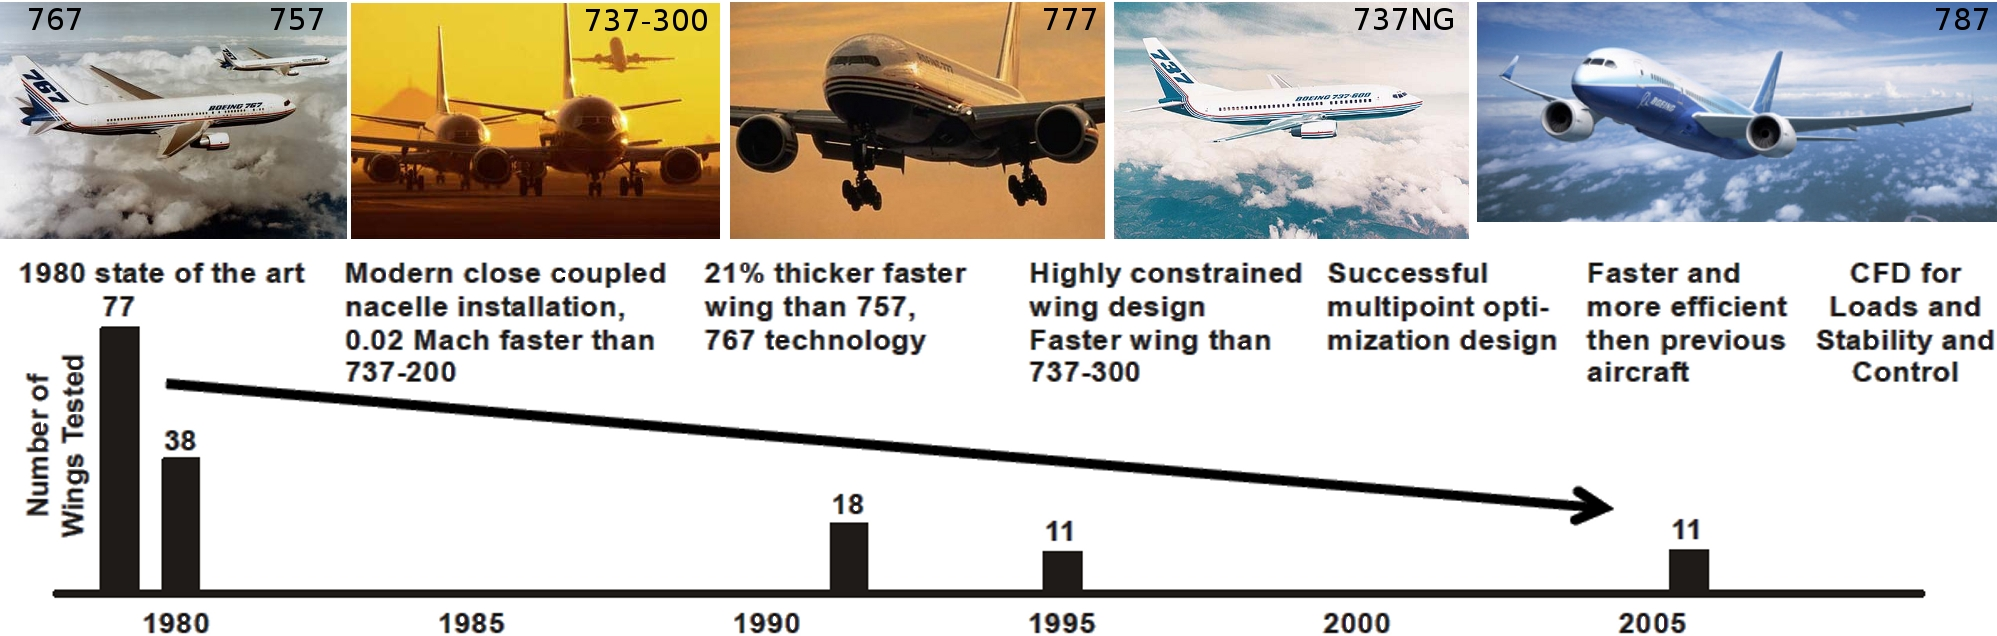
\includegraphics[width=1.0\linewidth]{fig-future/fig8.jpg}}
% --- end paragraph admon ---





% !split
\subsection*{The future: A new type of students}


% --- begin paragraph admon ---
\paragraph{}
\textbf{Computations (mastering and developing)  will play a central role in almost all aspects of scientific investigations and technological innovation}
% --- end paragraph admon ---




% --- begin paragraph admon ---
\paragraph{}
\textbf{Candidates who are capable of modeling and understanding complicated
systems, are in short supply in society}.
% --- end paragraph admon ---



% --- begin paragraph admon ---
\paragraph{}
We need students that  
\begin{itemize}
\item can handle large and demanding multi-disciplinary  projects. This requires structured thinking and good analytical skills and a thorough understanding of the problems to be solved 
\end{itemize}

\noindent
This knowledge makes the students unique on the labor market, a labor market which in the years to come will experience heavy automatization and massive loss of jobs.
% --- end paragraph admon ---






% !split
\subsection*{The challenges for the future}

% --- begin paragraph admon ---
\paragraph{}
We need to educate the next generation of 
science students with the knowledge, skills, and values needed to pose
and solve current and new scientific, technological and societal
challenges.
% --- end paragraph admon ---



% --- begin paragraph admon ---
\paragraph{}
This will lay the foundation for cross-disciplinary
educational, research and innovation activities. It will contribute to building a common cross-disciplinary
approach to key strategic initiatives, with important examples from fields like  \emph{Energy research, Materials science and  Life Science}.
% --- end paragraph admon ---











% !split
\subsection*{What we should do: create the Department  for Computational Science}

% --- begin paragraph admon ---
\paragraph{What we have and where we can arrive.}
\begin{itemize}
\item UiO's strength in computational science (education and research) will play an important role in  determining new research and educational directions

\item Exploiting this strength has the potential to make UiO a center of excellence for scientific innovation
\end{itemize}

\noindent
% --- end paragraph admon ---




% --- begin paragraph admon ---
\paragraph{How to achieve it.}
\begin{itemize}
\item Establish  a new center/department with focus on computational science and its applications to a wide range of fields (natural science, medicine, social sciences, humanities, applied research etc)

\item Hire ten (or more) young professors (age $< 40$) dedicated to innovative research and education where computations play a central role

\item Establish another ten professorships (or more) with  shared positions (position percentage  is flexible) between the  new department and the department of appartanence (physics, chemistry, etc etc).
\end{itemize}

\noindent
% --- end paragraph admon ---



\textbf{The process must start now} in order not to loose momentum.


% !split
\subsection*{Our takeaway messages}

% --- begin paragraph admon ---
\paragraph{}
\begin{itemize}
\item A successful research program cannot be disconnected from education and vice versa

\item Computing plays and will play an even more important role in future scientific and technological advances

\item An educational and research program which focuses on these issues needs to be established as soon as possible

\item The main aim in developing a good educational and research program is  that students should learn to realize their own potentials and creative power
\end{itemize}

\noindent
% --- end paragraph admon ---




% !split
\subsection*{The Computing in Science Education project, UiO educational prize in 2011}

% --- begin paragraph admon ---
\paragraph{}
The insights, ideas and thoughts presented here, would have been impossible or difficult to gain without discussions, exchange of ideas and much more over many years with colleagues involved in the \href{{http://www.mn.uio.no/english/about/collaboration/cse/}}{Computing in Science Education} project at UiO. These dear friends and colleagues  are 
\begin{itemize}
\item Hans Petter Langtangen, Informatics and Simula Research Laboratory

\item Knut Mørken, Mathematics

\item Arnt Inge Vistnes, Physics

\item Oyvind Ryan, Mathematics

\item Solveig Kristensen and Annik Myhre, Deans of Education, MN faculty

\item Hanne Sølna, Director of studies MN faculty

\item \textbf{And: all our fantastisc students who keep giving us new insights!}
\end{itemize}

\noindent
% --- end paragraph admon ---


Thanks for the attention.








% ------------------- end of main content ---------------


\printindex

\end{document}

